\lecture{Domanda variabile deterministica}{15~-~02~-~2026}
%
%
\section{Fondamenti e Modellazione del Problema}
In un contesto di gestione delle scorte, il flusso dei materiali avviene tra un Fornitore e un Reparto Produttivo, mediato da un Magazzino. L'obiettivo è gestire il livello di inventario $I_t$ bilanciando gli arrivi $a_t$ (forniture) e le uscite $u_t$ (consegne).

Ricordiamo che il livello dell'inventario (vedi sez. \ref{sec:dinamica_sim}) è definito da:
\[
    I_{t} = I_{t-1} + a_{t} - u_{t}
\]
\[
    I_{t}\geq 0, \quad \forall t \geq 0
\]
Il problema può essere formulato attraverso la \emph{Programmazione Lineare} (PL), con l'obiettivo di minimizzare i costi totali composti da:
\begin{itemize}
    \item \textbf{Costi di stoccaggio} ($h$): legati alla quantità tenuta a magazzino;
    \item \textbf{Costi di riordino/setup} ($A$): costi fissi ogni volta che si emette un ordine ($S_t=1$).
\end{itemize}
La funzione obiettivo è:
\[
    \min \sum_{t=1}^{T}hI_{t}+\sum_{t=1}^{T}AS_{t}
\]
\begin{align*}
    \text{s.t.} \quad I_{t} & = I_{t-1}+Q_{t}-D_{t}                 & \forall t \\
    Q_{t}                   & \leq MS_{t}, \quad M > 0              & \forall t \\
    S_{t}                   & \in \begin{Bmatrix} 0,1 \end{Bmatrix} & \forall t \\
    Q_{t}                   & \geq 0, \quad I_{0},I_{t} \geq 0      & \forall t
\end{align*}

dove troviamo:
\begin{multicols}{2}
    % \centering
    $ I_{t} $: Inventario alla fine del tb (\emph{time bucket}); \\
    $ Q_{t} $: Quantità da ordinare nel tb; \\
    $ S_{t} = 1$: Riordino nel tb; \\
    $ S_{t} = 0 $: Non riordino nel tb; \\
    $ h $: Costo di stoccaggio; \\
    $ A $: Costo di riordino; \\
    $ I_{0} $: Inventario iniziale.
\end{multicols}

Tuttavia, al crescere dell'orizzonte temporale, il numero di variabili e vincoli nel modello PL cresce notevolmente, rendendo necessario l'uso di altri approcci come euristiche o programmazione dinamica.

%
\section{Metodi Euristici}
Le euristiche sono regole empiriche e intuitive che forniscono soluzioni non necessariamente ottimali ma veloci da calcolare. In questi metodi, il costo di produzione puro viene trascurato perché la quantità totale prodotta per soddisfare la domanda è fissa indipendentemente dalla politica scelta:
\begin{enumerate}
    \item \emph{Lot for a Lot (L4L)};
    \item \emph{Fixed Order Quantity (FOQ)};
    \item \emph{Periodic Order Quantity (POQ)};
    \item \emph{Silver Meal};
    \item \emph{Part Period Balancing (PPB)}.
\end{enumerate}

%
\paragraph{Lot for a Lot} In ogni time bucket si ordina esattamente la quantità necessaria per quel periodo ($Q_t = D_t$): è ideale per industrie su domanda intermittente.
\begin{example}[L4L]\label{ex:l4l}
    Vedi figura \ref{fig:figl4l}:
    \begin{gather*}
        I_{0} = 0 \\
        A = 100 \text{\euro} \\
        h = 6 \frac{\text{\euro}}{\text{tb}}
    \end{gather*}
    Risoluzione:
    \[
        \text{Costo Totale} = \sum_{t=1}^{8}hI_{t}+\sum_{t=1}^{8}AS_{t} = 6 \cdot 0 + 100 \cdot 8 = 800
    \]
\end{example}
\begin{figure}
    \centering
    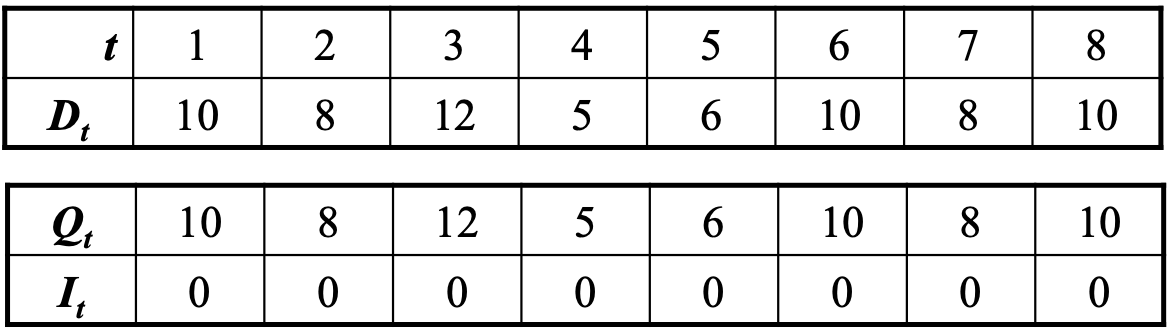
\includegraphics[width=0.5\linewidth]{assets/Screenshot 2026-02-15 at 16.09.57.png}
    \caption{Esercizio \ref{ex:l4l}}\label{fig:figl4l}
\end{figure}

%
\paragraph{Fixed Order Quantity} Si ordina una quantità fissa ($FOQ$) ogni volta che il magazzino non copre la domanda. La quantità è basata sulla formula dell'EOQ (Lotto Economico) usando la domanda media $\overline{D}$.
\[
    FOQ = \sqrt{\frac{2A\overline{D}}{h}}, \quad \overline{D} = \frac{1}{T}\sum_{t=1}^{T}D_{t}
\]
Si utilizza quando è vantaggioso avere lotti di dimensione costante.

%
\paragraph{Periodic Order Quantity} Si definisce un intervallo di tempo fisso di riordino. Si ordina la somma della domanda prevista per quell'intervallo.
\[
    POQ = \frac{EOQ}{D}, \quad EOQ = \sqrt{\frac{2A \overline{D}}{h}}, \quad \overline{D} = \frac{1}{T}\sum_{t=1}^{T}D_{t}
\]
Si utilizza quando è vantaggioso avere ordini periodici.

%
\paragraph{Silver Meal} Si calcolano i costi medi necessari a soddisfare la domanda di un numero crescente di time bucket fino a quando tali costi non divengono crescenti.
\[
    \min_{m}
    \begin{bmatrix}
        \overline{TC}(t,t+m)
    \end{bmatrix} =
    \min_{m}
    \begin{bmatrix}
        \frac{1}{m+1} \begin{pmatrix}
                          A + \sum_{i=t}^{t+m}(i-t)hD_{i}
                      \end{pmatrix}
    \end{bmatrix}
\]

%
\paragraph{Part Period Balancing} Si tenta di uguagliare i costi di ordinazione ($A$) con i costi di stoccaggio sui vari time bucket.
\[
    \min_{m}
    \lvert T_{c} (t,t+m) \rvert =
    \min_{m}
    \lvert A - \sum_{i=t}^{t+m}(i-t)hD_{i} \rvert
\]

%
\section{Programmazione dinamica}
Qualunque soluzione ottima è caratterizzata dalla condizione di ottimalità $ S_{t} \cdot I_{t} = 0 $, ovvero si ordina solo quando il magazzino è vuoto.

La soluzione ottima fino al time bucket $ t $ non dipende da ciò che avviene
nell'intervallo di tempo $ t+1 $, ovvero si può lavorare con un orizzonte
temporale finito.
%
\subsection{Algoritmo Wagner-Whithin}
Questo algoritmo di Programmazione Dinamica (1958) garantisce l'individuazione della soluzione ottima assoluta.

\newpage
\begin{multicols}{2}
    % \begin{enumerate}[leftmargin=2.3cm, label=Passo \arabic*.]
    %     \item $ t=1,~I_{1}=0 $. Si produce la quantità $ D_{1} $. $ T_{C1} = A_{1} $
    %     \item $ t=1,~I_{1}=0 $. Si produce la quantità $ D_{1} $.
    %     \item
    % \end{enumerate}

    \begin{stepbox}
        $t=1,~I_{1}=0 $. \\
        Si produce la quantità $ D_{1} $. \\
        $ T_{C1} = A_{1} $
    \end{stepbox}

    \begin{stepbox}
        $ t=2,~I_{2}=0 $. \\
        Si sceglie il costo minimo tra le due possibilità:
        \begin{enumerate}[label=\alph*)]
            \item Si produce $ D_{2} $ in $ t=2 $. \\ $ T_{C2} = T_{C1} + A_{2} $.
            \item Si produce $ D_{2} $ in $ t=1 $. \\ $ T_{C2} = A_{1} + h_{1}D_{2} $.
        \end{enumerate}
    \end{stepbox}

    \begin{stepbox}
        $ t=3,~I_{3}=0 $.\\
        Si sceglie il costo minimo tra le tre possibilità:
        \begin{enumerate}[label=\alph*)]
            \item Si produce $ D_{3} $ in $ t=3 $. \\ $ T_{C3} = T_{C2} + A_{3} $.
            \item Si produce $ D_{3} $ in $ t=2 $. \\ $ T_{C3} = T_{C1} + A_{2} + h_{2}D_{3} $.
            \item Si produce $ D_{3} $ in $ t=1 $. \\ $ T_{C3} = A_{1} + h_{1}D_{2} + (h_{1}+h_{2})D_{3} $.
        \end{enumerate}
    \end{stepbox}

    \begin{stepbox}
        $ t=4,~I_{4}=0 $.\\
        Si sceglie il costo minimo tra le quattro possibilità:
        \begin{enumerate}[label=\alph*)] % chktex 9 chktex 10
            \item Si produce $ D_{4} $ in $ t=4 $. \\ $ T_{C4} = T_{C3} + A_{4} $.
            \item Si produce $ D_{4} $ in $ t=3 $. \\ $ T_{C4} = T_{C2} + A_{3} + h_{3}D_{4} $.
            \item Si produce $ D_{4} $ in $ t=2 $. \\ $ T_{C4} =  T_{C1} + A_{2} + h_{2}D_{3} + (h_{1}+h_{2})D_{3} + (h_{1}+h_{2}+h_{3})D_{4} $.
            \item Si produce $ D_{4} $ in $ t=1 $. \\ $ T_{C4} =  A_{1} + h_{1}D_{2} + (h_{1}+h_{2})D_{3} + (h_{1}+h_{2}+h_{3})D_{4} $.
        \end{enumerate}
    \end{stepbox}
\end{multicols}

La condizione di ottimalità $ S_{t} \cdot I_{t}=0 $ garantisce che in una soluzione ottima la scelta di quando produrre la quantità $ D_{t} $ non possa scendere al di sotto dell'ultimo intervallo in cui è stato deciso di produrre. In generale, essendo $ t-r $ l'ultimo time bucket in cui si è avuta produzione: % chktex 17
\[
    T_{Ct}^{*} = \min \left\{
    \begin{array}{ll}
        T_{Ct-1}^{*} + A_{t}                  \\
        T_{Ct-2}^{*} + A_{t-1} + h_{t-1}D_{t} \\
        \dots                                 \\
        T_{Ct-(r+1)}^{*} + A_{t-r} + h_{t-r}D_{t-r+1} + \cdots + (h_{t-r}+h_{t-r+1}+\cdots+h_{t=1})D_{t}
    \end{array}
    \right.
\]